
%
%
%
%
%
%
%
\chapter{Implementation Details }
\section{Preparing and Reading in data}
When using our provided data importing functions we expect the data to be stored in two folders one for the raw image files and one folder for the ground truth mask. These folders must be labled "Images" and "GroundTruth" respectively. Both raw images and ground truth can be in .bmp, .tif or .png formats but the format has to be uniform throughout a dataset. Additionally it should be noted that the ground truth mask is mapped to its image only by file name so in the end the images folder and the groundtruth folder must have the same number of files with the same set of names. Ground truth masks labels are read in per pixel color or grayscale value, the ground-truth mask should be considered a space indexed label mapping so each label must have exactly one value here, which also means these files should be much smaller than the image files. The data location is specified by the input argument "dataDir=".
\subsection{Caching}
If the user chooses to run our preprocessing functions for creating super-pixels, extracting features and constructing the graph, then all of these will be cached on disk in the same folders where the data resides. The caches are performed for each image individually and are named after the raw image of origin as well as some information about what options where used when creating this cache. With this very simple caching system we prevent the user from having to recompute every image in the event of a crash, or when changing a few parameters for later portion of the pipeline. If the user wishes to rewrite the cache without checking if there are matching flags in the files one should specify the input argument "recompFeat=true" or the user can change the "runName=" input argument as it will a new set of caches while leaving the old ones as is. The files ending in ".mask" in the Images folder contain the mapping between pixel index to super-pixel id. Files ending in ".graph2" contain the completed graph structure of the associated image, I.E. nodes which only save their own features and the node id's of their neighbors. Files ending in ".classCount" , ".colorlabelmapping2" and ".transProb" contain the class frequency count, map between colors used in the groundtruth files and internal label id and the transition probabilities between labels respectively. The files ending in ".labels2" contain the cache for the true labelled graph of these training dataset. 


\subsection{Feature Standardization}
Standardizing features is important especially when some features are degrees of magnitude larger than others, for example when including \inputArgs{featAddIntensityVariance} and \inputArgs{featHistSize}. 




\section{Features}
Since our data is split up into non uniformly shaped super-pixels we could not use off the shelf feature functions. We implemented some basic features like color or intensity histograms, Co-occurance matrix, and some features based on the super-pixel graph structure like the sum of neighbor histograms, in neighbourhood intensity uniqueness and some others. All these features are computed after the super-pixel bounds have been determined. Most of the features are extracted by once running overall pixels in the image and adding to some moving average of the feature indexed by the super-pixel id of that corresponding pixel. If using our graph construction script \codeInLine{genGraphFromImages()} the features are specified as arguments into either \codeInLine{featureFn} or \codeInLine{afterFeatreFn}. As the name implies afterFeatureFn is run after the graph is constructed and provides the feature functions with the graph edge information, featureFn is for unary features only. If also using our start-up main \codeInLine{ch.ethz.dalab.dissolve.examples.neighbourhood.runReadTrainPredict} then the feature functions are constructed for the user who only has to specify which features are desired. 
\subsection{Predefined Feature List}
All below features can be specified in the runtime arguments of \codeInLine{runReadTrainPredict} for color, greyscale , 2d and 3d image datasets. 

\begin{description}
\item[\inputArgs{featIncludeMeanIntensity}] Averages all pixels assigned to a super-pixel into one mean intensity. For color this mean intensity is the corresponding converted greyscale intensity. This feature may also be added to the metadata of a node such that the datadependent pairwise models can use it.  
\item[\inputArgs{featHistSize}] If set above Zero we construct a normalized histogram of colors or gray scale intensities with equally sized bins. Bin sizes are always $\frac{255}{featHistSize}$. The color version of this histogram constructs bins per color dimension and but keeps the same number of bins specified, hence for color \inputArgs{featHistSize} must be divisible by three.
\item[\inputArgs{featUseStdHist}] Will construct non histigrams with non uniform bin sizes. Rather it initially computes a global distribution of intensities and constructs bins which should contain approximately equal datapoints. \inputArgs{featHistSize} is still used to specify the number of bins but only the standardized bins are used in the features. The bin sizes are computed once for the whole dataset and are ofcourse not adjusted for new data hence the training set must be sufficiently large for the distribution to be accurate. 
\item[\inputArgs{featCoOcurNumBins}] Co-occurance matrices are constructed again binning all pixels into uniformly sized ranges of the intensity spectrum and then counting all occurrences of a pixel binned to bin $A$ neighbouring a pixel in bin $B$. Again the number of bins must be divisible by three if used on color data. One can specify exactly which kind of neighborhood should be used by default we only consider one pixel hop and no diagonals, to change this one must alter the feature function call with different $directions$ input. 
\item[\inputArgs{featAddOffsetColumn}] This will simply add a column of ones into the feature vector giving the SSVM one more degree of freedom for its decision boundary. 
\item[\inputArgs{featAddIntensityVariance}] calculates pixel intensity variance per super-pixel, for color images this is again the converted greyscale value $\frac{Red}{3}+\frac{Green}{3}+\frac{Blue}{3}$. 
\item[\inputArgs{featUniqueIntensity}] Computes mean intensities and variances if not yet computed for all super-pixels then measures the number of standard deviations away from the mean of a super-pixels one hope neighbourhood its own intensity is. 
\item[\inputArgs{featUnique2Hop}] Same as \inputArgs{featUniqueIntensity} but using a 2 edge hope neighbourhood. 
\item[\inputArgs{featNeighHist}] Computes histograms per super-pixels as in \inputArgs{featHistSize} and then sums all the histograms of neighboring super-pixels not include the data from the super-pixels own space and then normalizes. \inputArgs{featHistSize} again determines the size of the bins used here. 
\item[\inputArgs{featAddSupSize}] The count of the number of voxels assigned to a particular super-pixel. 

\end{description}



\section{Additional Runtime Arguments }

Critical 
\begin{description}
\item[\inputArgs{useNaiveUnaryMax}] Setting this to true will result in dissolve using the simple per node max decoding inside the oracle function. See section \ref{sec:unaryMax}.
\item[\inputArgs{useMF}] If Set to true, dissolve will use the Mean Field appoximation to solve the max oracle problem. See Section \ref{sec:meanField}
\item[\inputArgs{modelPairwiseDataDependent}] If set to true, the max oracle will be performed on a CRF where the pairwise potentials are dependent on the label but also a function of the two super-pixels features. This model was only implemented for Loopy Beliefe Propagation decoding.  See Section \ref{sec:dataDep}
\item[\inputArgs{mfTemp}] Specify any Double value for use as the Temperature paramater in the Mean Field decoding. See Section \ref{sec:meanField}
\item[\inputArgs{useLoopyBP}] If set to true, Loopy Belief Propagation will be used for the max-oracle function. See \ref{eq:loopybp
\item[\inputArgs{loopyBPmaxIter}] Loopy Belief propagation iterations before returning the max-oracle decoding. Training time scales linearly with the number of iterations. 
\item[\inputArgs{useRandomDecoding}] For debugging and comparison purposes we have included a max-oracle which returns a random $\yVect$. 
\item[\inputArgs{roundLimit}]


\item[\inputArgs{onlyUnary}] Used to specify if the max oracle should run decoding on a CRF with only unary potentials, see Section \ref{sec:crfvarations}
\item[\inputArgs{lambda}] The regularizing parameter see section  \ref{sec:Lambda}
\item[\inputArgs{doLineSearch}] 
\item[\inputArgs{numClasses}] The expected range of labels.
\item[\inputArgs{isColor}] Set to true if the data being read in is using RGB leave false if data is grey scale. 
\item[\inputArgs{useClassFreqWeighting}] If set to true the lossFn will not be a zero-one loss but rather every missclassificaiton is counted as one inverse class frequency.  This is import to set as true if using dataset which has large imbalance in the label counts. 
\item[\inputArgs{superpixelSize}] Set to an Integer greater than zero this is the $S$ parameter in our SLIC implementation. See Section \ref{sec:slicAlgo}
\item[\inputArgs{slicCompactness}]  Set a double value greater than zero, this corresponds to the $M$ paramater in SLIC. See Section \ref{sec:slicParams}
\item[inputArgs{dataFilesDir}] The path to your training raw images and ground truth. In this folder we expect a subfolder named GroundTruth and one named Images. The user can also specify these seperatly with \inputArgs{imageDataFilesDir} and \inputArgs{groundTruthDataFilesDir}
\item[\inputArgs{numberOfCoresToUse}]


\end{description}

\section{Example Run}

\todo{put code for some example runs and file structures}
For viewing the predicted labels we recommend UCSB's bioView3D \cite{bio3dViewer}. 

Optional
\begin{description}
\item[\inputArgs{trainTestEqual}] If set to true, the preprocessor will not reserve any data for testing but rather train on all possible data. 
\item[\inputArgs{squareSLICoption}] If set to true, the SLIC preprocessing will simply produce square super-pixels. Run time for these super-pixels is only $\mathcal{O}(n)$. 
\item[\inputArgs{LOSS\_AUGMENTATION\_OVERRIDE }]If set to true optimization the objective without considering loss between graph labels. As in $\min_{\weightVec} \frac{\lambda}{2} ||\weightVec||^2 \frac{1}{n} \sum_{i=1}^n \max_{y in \ySpace} \langle \weightVec , \jointFeatureMap \rangle$
\item[\inputArgs{initWithEmpiricalTransProb}] Will precalculate the class transition probability table and initialize the pairwise section of the $w$ to these values. 
\item[\inputArgs{dbcfwSeed}] A random seed used inside BCFW setting this to non -1 value will allow for deterministic output. 
\item[\inputArgs{runName}] A simple string used in logging and in the cache files.
\item[\inputArgs{checkpointFreq}] 
\item[\inputArgs{dataGenSparsity}] The desired percentage of the ground truth which is background when generating synthetic data. See section \ref{sec:synthDataGen}
\item[\inputArgs{dataNoiseOnlyTest}] If set to true the data generated will only add the specified noise to the test set not the training dataset. 


\item[\inputArgs{dataGenCanvasSize}] Number of pixel rows/columns per image being generated. Images are always square. 
\item[\inputArgs{dataRandSeed}] A seed value for the random number generators used in the data synthesis functions. If set to a non -1 value then the data generation is deterministic.  Allowing experiments to be run over different machines without having to transfer the data. 
\item[\inputArgs{dataGenSquareSize}] The size of the super-squares used in synthetic data generation, see Section \ref{sec:synthDataGen}
\item[\inputArgs{dataGenSquareNoise}] A decimal between 0.0 and 1.0 specifying how much SuperSquareShift noise should be added, see Section \ref{sec:synthDataGen}
\item[\inputArgs{dataGenHowMany}] An Integer specifying how many images to generate. 
\item[\inputArgs{dataGenOsilNoise}] A decimal between 0.0 and 1.0 specifying how much  OscillationNoise noise should be added, see Section \ref{sec:synthDataGen}
\item[\inputArgs{dataGenGreyOnly}] If Set to true, the synthetic data generated will only have features in gray scale values.
\item[\inputArgs{dataGenEnforNeigh}] Setting this value between 0.0 and 1.0 specifies the probability with which two labels are allowed to be neighbors. Addtionally one must set \inputArgs{dataGenEnforNeigh} to true for this setting to take effect.  see Section  \ref{sec:synthDataGen}
\item[\inputArgs{recompFeat}]
\item[\inputArgs{maxColorValue}]
\item[\inputArgs{dataDepUseIntensity}]
\item[\inputArgs{numDataDepGraidBins}]
\item[\inputArgs{dataDepUseIntensityByNeighSD}]
\item[\inputArgs{dataDepUseIntensityBy2NeighSD}]
\item[\inputArgs{dataDepUseUniqueness}]
\item[\inputArgs{dataDepUseUniquenessInOtherNeighbourhood}]
\item[\inputArgs{slicMinBlobSize}]
\item[\inputArgs{standardizeFeaturesByColumn}]

\item[\inputArgs{alsoWeighLossAugByFreq}]
\item[\inputArgs{splitImagesBy}]
\item[\inputArgs{optimizeWithSubGraid}]
\item[\inputArgs{pairwiseModelPruneSomeEdges}]
\item[\inputArgs{slicSimpleEdgeFinder}]
\item[\inputArgs{filterOutImagesWithOnlyOneLabel}]
\item[\inputArgs{leaveOneOutCrossVal}]
\item[\inputArgs{leaveOutCVmaxIter}]
\item[\inputArgs{logOracleTiming}]


\item[\inputArgs{enableOracleCache}] 
\item[\inputArgs{oracleCacheSize}]
\item[\inputArgs{H}]
\item[\inputArgs{sampleFrac}]
\item[\inputArgs{sampleWithReplacement}]
\item[\inputArgs{enableManualPartitionSize}]
\item[\inputArgs{NUM\_PART}]
\item[\inputArgs{debug}]
\item[\inputArgs{debugWeightUpdate}]
\item[\inputArgs{debugMultiplier}]
\item[\inputArgs{sparse}]

\item[\inputArgs{debugPrintSuperPixImg}] If set to true, after training is complete \codeInLine{ch.ethz.dalab.dissolve.examples.neighbourhood.runReadTrainPredict} will print a colored overlay ontop of the input image indicating the predicted labels per pixel. This function will also print out the correct label for comparison. It assumes that 
\item[\inputArgs{compPerPixLoss}] When using a folder \codeInLine{../data/debug} exists. \codeInLine{ch.ethz.dalab.dissolve.examples.neighbourhood.runReadTrainPredict} this parameter determines if after training the model will be tested on the reconstructed per pixel labels in addition to the standard per pixel error reporting. 

\end{description}


\section{Synthetic Data Generation} \label{sec:synthDataGen}
In order to intuitively show where the pairwise models have an advantage over a non structured approach we constructed a series of synthetic data generation functions. \todo{TODO Pseudocode styling on the following} [ 1. Randomly choose a true color per label. 2. Divide the image into a grid of “super-squares” and randomly assign a label to each super square 3. paint each real pixel with the true color plus all types of noise for this coordinate and project back into RGB or 8-Bit Greyscale space. The ground truth is generated in the same way with the same colors just without the noise added] [ We have 3 types of noise 1. SuperSquareShift, where in we equally shift all pixels in this supersquare in a random color direction. 2. WhiteNoise, simply add a random color per pixel 3. OscillationNoise, this noise is base on the x,y coordinates, the S chosen for that experiment and a random phase shift chosen per image. osilatingNoise*(cos(x*/osilationWaveLength+rPhaseX)*cos(y*/osilationWaveLength+rPhaseY)+1)*255/2 ] [ Finally we also add a restriction on which labels can be neighbours this is randomly chosen between possible pair of labels with the probability labled “dataGenNeighProb”. Note that Label zero is considered the background and can be adjacent to any other label]. See Figures : (\ref{fig:squareNoise}, \ref{fig:whiteNoise} and \ref{fig:osIlNoise}) for visual examples of these types of noise and Figure \ref{fig:allNoise} for the all together as a typical dataset. The 3 types of noise are needed to make the unary model based classifiers less powerfull because if they are too accurate themselves it is unlikely that the SSVM would add any norm to the weight vector to use the unnecessary pairwise term. The OscillationNoise is set at a wavelength proportional to S such that adjacent super pixels inside one super-square will always have different amount of noise added. The  dataGenNeighProb is used to make the transition probability more sparse and hence easier to learn making the difference between unary and pairwise models more evident. Figure \ref{fig:dataGenNeighExp} is an example of  a dataset which has \inputArgs{dataGenNeighProb=0.3} in contrast to Figures \ref{fig:squareNoise}, \ref{fig:whiteNoise} and \ref{fig:osIlNoise} which have \inputArgs{dataGenNeighProb=1.0}.

\begin{figure}
  \centering
  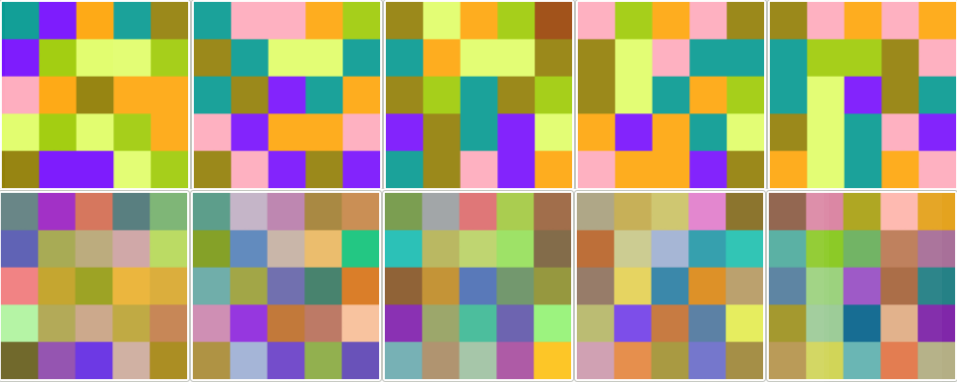
\includegraphics[width=0.8\textwidth]{images/generatedData__none_color_20_150_0_01_8_0_4_0_0_0_0_1_0_10_20___.png}
  \caption{ An example of SuperSquareShift noise, the top row is the true ground truth and the bottom row is the image data used for features with SuperSquareShift=0.4 included.  } 
  \label{fig:squareNoise}
\end{figure} 

\begin{figure}
  \centering
  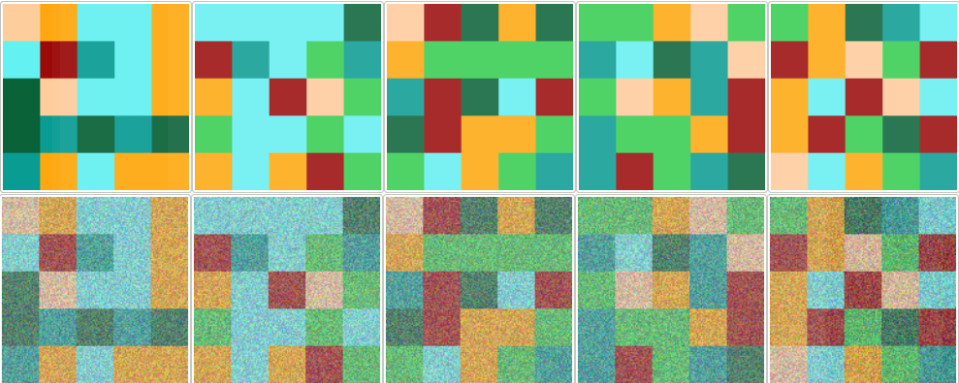
\includegraphics[width=0.8\textwidth]{images/generatedData__none_color_20_150_0_01_8_0_0_0_4_0_0_1_0_10_12___.png}
  \caption{ An example of WhiteNoise, the top row displays the groundtruth and the bottom are the feature images with whtieNoise=0.4 added. } 
  \label{fig:whiteNoise}
\end{figure} 

\begin{figure}
  \centering
  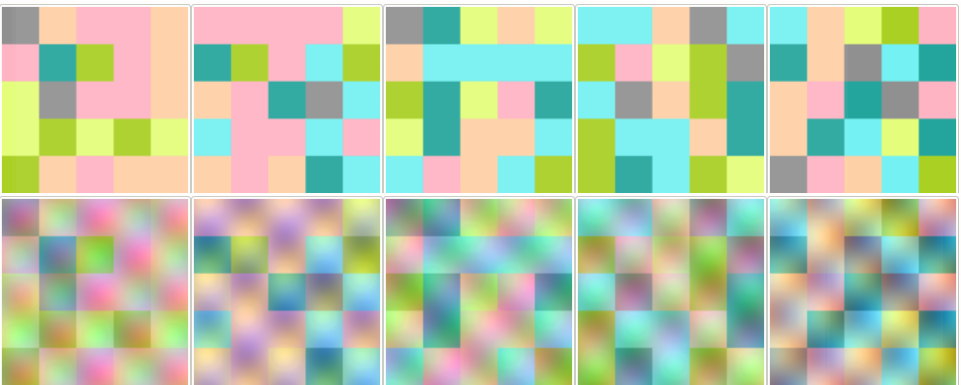
\includegraphics[width=0.8\textwidth]{images/generatedData__none_color_20_150_0_01_8_0_0_0_0_0_4_1_0_10_12___.png}
  \caption{ And example of OsilationNoise, the top row displays the groundtruth and the bottom row are the feature images with osilationNoise=0.4 added. } 
  \label{fig:osIlNoise}
\end{figure} 

\begin{figure}
  \centering
  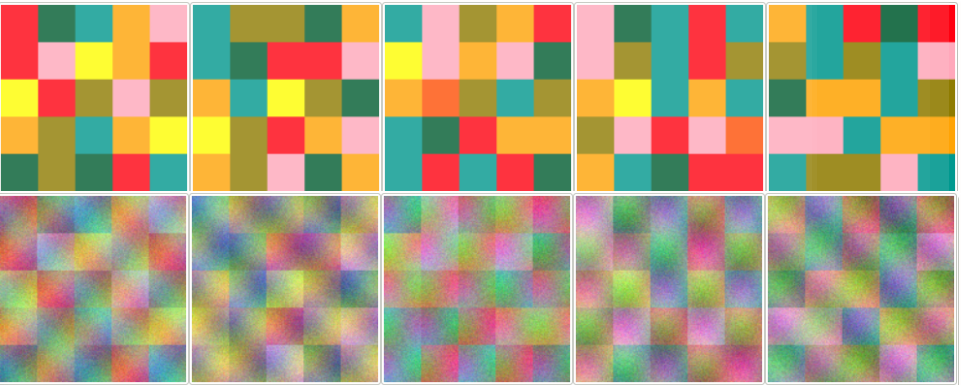
\includegraphics[width=0.8\textwidth]{images/generatedData__none_color_20_150_0_01_8_0_05_0_35_0_45_1_0_10_11___.png}
  \caption{  An example of all types of noise. The groundtruth is in the top row an the feature images are in the bottom row with the following nois added: Super-Square-shift=0.05, WhiteNoise=0.35 and OsilationNoise=0.45.} 
  \label{fig:allNoise}
\end{figure} 

\begin{figure}
  \centering
  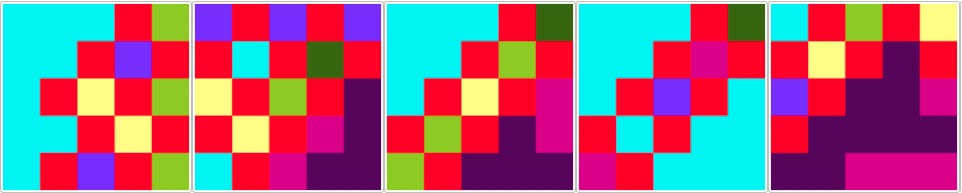
\includegraphics[width=0.8\textwidth]{images/DataGenNeighProb_0_3_seed13.png}
  \caption{  An example dataset showing groudataGenNeighProb=0.3, it can be contrasted to \ref{fig:allNoise} where the ground truth was generated with groudataGenNeighProb=1.0. We can see that in the above image some colors never occur next to each other.  } 
  \label{fig:dataGenNeighExp}
\end{figure} 


%
